% Printed 103; principal PDF 110; Google PDF 114.
\par\clearpage

\vspace*{.09\textheight}
\begin{center}{\LARGE P\,O\,S\,T\,H\,U\,M\,O\,U\,S\ P\,A\,P\,E\,R\,S.}\end{center}
\vspace{.05\textheight}
\begin{center}
[1.]\\[.5ex]
Reduction of the spherical triangle angles \(A,B,C\) to the chord angles\\
\(\mathfrak{A},\mathfrak{B},\mathfrak{C}\).
\end{center}

\noindent\begin{minipage}[t]{.65\textwidth}
\setlength{\parindent}{1.5em}
\indent Circumscribe a circle about the triangle.\\
Thus the 3 quadrilaterals the measure [of the corrections].

Let
\[
\frac{a}{\sin A}=\frac{b}{\sin B}=\frac{c}{\sin C}=\nu
\]
\[
\nu a\cos A=\alpha,\quad \nu b\cos B=\beta,\quad \nu c\cos C=\gamma.
\]
\noindent Then the reductions are
\[
\frac{\beta+\gamma}{8},\quad
\frac{\alpha+\gamma}{8},\quad
\frac{\alpha+\beta}{8}.
\]
\end{minipage}\hfill
\begin{minipage}[t]{.33\textwidth}
\vspace{0pt}\centering
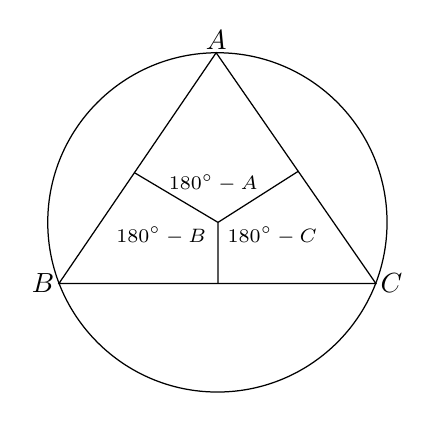
\begin{tikzpicture}[x=1.55cm,y=1.55cm,line width=.45pt]
\coordinate (A) at (-.01,1.39);
\coordinate (B) at (-1.298,-.50);
\coordinate (C) at (1.298,-.50);
\coordinate (O) at (.005,0);
\path (A)--(B) coordinate[pos=.52] (AB);
\path (A)--(C) coordinate[pos=.514] (AC);
\path (B)--(C) coordinate[pos=.502] (BC);
\draw (0,0) circle[radius=1.39];
\draw (A)--(B)--(C)--cycle;
\draw (AB)--(O)--(AC) (O)--(BC);
\node[above,inner sep=1pt] at (A) {\(A\)};
\node[left,inner sep=1.5pt] at (B) {\(B\)};
\node[right,inner sep=1.5pt] at (C) {\(C\)};
\node[font=\scriptsize,inner sep=0pt] at (-.035,.32) {\(180^\circ-\mathfrak A\)};
\node[font=\scriptsize,inner sep=0pt] at (-.46,-.11) {\(180^\circ-\mathfrak B\)};
\node[font=\scriptsize,inner sep=0pt] at (.45,-.11) {\(180^\circ-\mathfrak C\)};
\end{tikzpicture}
\end{minipage}
\par\bigskip

\begin{center}
[2.]\\[.5ex]
{[Condition for 3 points on the surface of a sphere}\\
to lie on a great circle.]
\end{center}

The condition for three points on the surface of a sphere whose
respective longitudes and latitudes are
\[
\begin{array}{l}
L,\ B\\
L',\ B'\\
L'',\ B''
\end{array}
\]
\noindent to lie on a great circle is given by the equation
\[
\operatorname{tang}B\sin(L'-L'')+\operatorname{tang}B'\sin(L''-L)+
\operatorname{tang}B''\sin(L-L')=0.
\]

\begin{center}\rule{.18\textwidth}{.4pt}\end{center}

% Printed 104; principal PDF 111; Google PDF 115.
\par\clearpage
\noindent\makebox[12mm][l]{\fontsize{13}{16}\selectfont 104}\makebox[\dimexpr\linewidth-24mm\relax][c]{\scriptsize\textbf{REMARKS.\quad REDUCTION OF THE SPHERICAL TRIANGLE ANGLES ETC.}}\makebox[12mm][r]{}\par\medskip

\vspace*{.11\textheight}
{\small
\begin{center}\textbf{REMARKS.}\end{center}

Note [1] is entered in a calculation notebook for the Hanoverian arc measurement. \textsc{Gauss}
here gives the values \(\frac{\beta+\gamma}{4}\), \(\frac{\alpha+\gamma}{4}\), \(\frac{\alpha+\beta}{4}\) for the corrections. The reduction of \(A\) to \(\mathfrak A\) can be obtained
from the equation
\[
\cos\mathfrak A=\sin\frac b{2r}\sin\frac c{2r}
+\cos\frac b{2r}\cos\frac c{2r}\cos A,\quad (r=\text{radius of the sphere})
\]
\noindent by expanding it. The expansion begins with
\[
A-\mathfrak A=\frac1{4rr}\,.\,\frac{bc}{\sin A}
-\frac1{8rr}(bb+cc)\operatorname{cotang}A\ldots
\]
\noindent and if we restrict ourselves to terms of second order, we may set
\[
bb+cc=aa+2bc\cos A
\]
\noindent to obtain
\[
A-\mathfrak A=\frac1{8rr}(2bc\sin A-aa\operatorname{cotang}A)
=\frac1{8rr}(bb\operatorname{cotang}B+cc\operatorname{cotang}C).
\]
\noindent The same result follows by noting that \(A-\mathfrak A\) equals the excess of the spherical
quadrilateral whose vertices are the pole of the triangle, the feet of the perpendiculars from this pole to sides
\(b\) and \(c\), and the point \(A\).

Note [2] is on the last leaf of \textsc{Gauss}'s copy of
“Analytischen Trigonometrie von G. S. \textsc{Klügel}. Braunschweig 1770.” According to a lecture by \textsc{Gauss}
entitled “Anleitung zur höhern Geodäsie,” of which a written record survives, the derivation of the condition
equation given in [2] rests on the fact that when
\[
\begin{aligned}
m&=n\sin(\varphi-\Phi)\\
m'&=n\sin(\varphi'-\Phi)\\
m''&=n\sin(\varphi''-\Phi)
\end{aligned}
\]
\noindent one has
\[
m\sin(\varphi'-\varphi'')+m'\sin(\varphi''-\varphi)+m''\sin(\varphi-\varphi')=0
\]
\noindent Now let \(i\) be the angle of inclination of the plane of the great circle to the equatorial plane, and
let the longitudes \(L-L_0\), \(L'-L_0\), \(L''-L_0\) be reckoned from the meridian passing through the intersection of the two planes.
Then we have
\[
\begin{aligned}
\operatorname{tang}B&=\operatorname{tang}i\sin(L-L_0)\\
\operatorname{tang}B'&=\operatorname{tang}i\sin(L'-L_0)\\
\operatorname{tang}B''&=\operatorname{tang}i\sin(L''-L_0).
\end{aligned}
\]
\par\hfill\textsc{Krüger, Börsch.}\hspace{.06\textwidth}\par
}
\begin{center}\rule{.24\textwidth}{.4pt}\end{center}

